\section{Struttura delle galassie a spirale}\label{sec:struttura-delle-galassie-a-spirale}
Analizziamo ora la struttura delle galassie a spirale: i dischi di spirale sono sempre in rotazione attorno al centro galattico. In quasi tutti i casi i bracci ruotano con bracci “trailing”, solo in pochissime galassie si hanno “leading arms” (fare riferimento alla figura~\ref{fig:trailing-leading arms}): la forma a spirale quindi data dal materiale che viene trascinato dai bracci ma che si muove con velocità diverse. Infatti NON si ha rotazione rigida: la velocità angolare NON è la stessa in tutti i punti del disco. Si ha invece rotazione differenziale, quindi le stelle più vicine al centro ruotano con velocità più elevate; in genere la velocità tangenziale è la stessa indipendentemente dalla distanza dal centro, quindi le regioni più esterne hanno velocità angolare $\omega = V/r$ minore rispetto a quelle più vicine al centro. Questo significa che le stelle delle regioni più lontane dal centro impiegheranno decisamente più tempo per compiere un'orbita rispetto a quelle più vicine al centro.

\begin{figure}
    \centering
    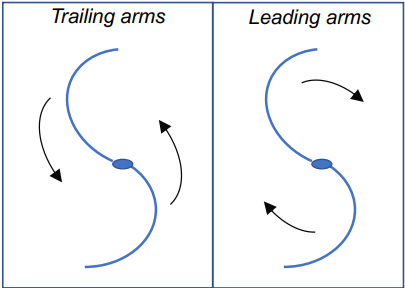
\includegraphics{immagini/trailing-leading-arms.png}
    \caption[width = 0.5 \textwidth]{Differenza tra "trailing arms" e " leading arms": nel primo caso i bracci sono trascinati dalla rotazione, mentre nel secondo guidano e anticipano la rotazione.}
    \label{fig:trailing-leading arms}
\end{figure}

In seguito a questa osservazione nasce il cosiddetto "dilemma del winding", mostrato in figura~\ref{fig:winding-dilemma}: se i bracci fossero fatti da materia, allora dovrebbero avvolgersi attorno al centro galattico in tempi scala più corti dell’età della galassia stessa (dopo poche decine di rotazioni). Questo però comporterebbe la perdita dei bracci, che risulterebbero tutti avvolti su se stessi, ma non è quello che noi osserviamo; infatti siamo in grado di osservare bracci a spirale anche per galassie molto antiche. La risposta quindi è che questo “arrotolamento” non c’è anche se è presente rotazione differenziale. Ma perché non c'è?

\begin{figure}
    \centering
    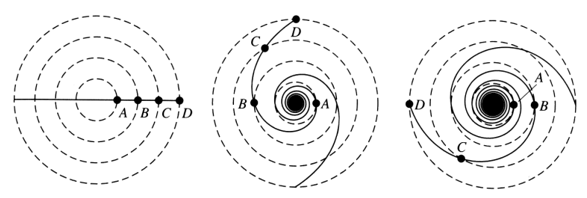
\includegraphics{immagini/winding-dilemma.png}
    \caption[width =\textwidth]{Dilemma del winding: se i bracci delle galassie fossero di materia dovrebbero pian piano arrotolarsi sul centro della galassia stessa.}
    \label{fig:winding-dilemma}
\end{figure}

La soluzione a questo quesito è basata sulla teoria di onda di densità di Lin: il fatto è che i bracci di spirale non sono materiali (quindi non sono composti da un insieme di gas e stelle che si muovono sempre insieme), ma sono generati da un’onda di densità, un’onda quasi-statica e molto duratura nel tempo. La galassia può essere pensata come un disco di materiale che ruota, attraversato da un’onda in compressione che ruota a sua volta ma a una velocità inferiore del disco materiale, creando così dei picchi di densità che sono quelli che chiamiamo bracci della spirale. I bracci di spirale sono perciò i luoghi di densità più elevata (e quindi la buca di potenziale è più profonda), ma NON sono composti sempre dalla stesse stelle! Si può fare un'analogia al caso delle macchine bloccate nel traffico: le zone dove c'è traffico sono quelle con maggiore densità di macchine e dove queste saranno costrette a trascorrere più tempo. Una volta superata la zona però la macchina se ne va e al suo posto ce ne saranno altre. Allo stesso modo le stelle e il gas, durante la loro orbita attraversano queste zone di più alta densità restandoci più a lungo ma pian piano escono e vengono sostituite da altre. Di conseguenza lo spazio fra i diversi bracci delle galassie non è vuoto e i bracci sono solo i luoghi dove le stelle della galassia trascorrono la maggior parte del tempo della loro orbita.

Questo modello spiega anche perché si ha formazione stellare lungo i bracci: quando le stelle e i gas entrano nell’onda si crea una regione di compressione che, per il criterio di instabilità di Jeans TEMP (che dice che le stelle si formano più facilmente in regioni di alta densità), fa sì che la formazione stellare sia favorita.

Un'altra cosa che a questo punto è naturale chiedersi è da cosa siano generate queste onde di densità? La risposta non è ancora chiara, ma si ipotizza che ci siano mancanze di simmetria iniziali nel disco, ad esempio legate al processo di formazione delle galassie, che prevedere l’interazione con altre galassie (quindi potrebbe esserci una galassia molto grande che interagisce con una piccolina a formare la galassia finale che in quella zona presenterà un zona a più alta densità).
